\section{Procedimento \& Analisi Dati}

Nell'ottica geometrica si usano le leggi del costruttore di lenti e dei punti coniugati.
Tali leggi si basano sulle ipotesi di raggi parassiali e lenti sottili, che dobbiamo quindi supporre verificate
nel nostro apparato sperimentale. Una parte dell'esperienza (quella relativa all'abberrazione sferica)
è dedicata alla misura dei limiti di tali approssimazioni.

\begin{figure}[b!]
	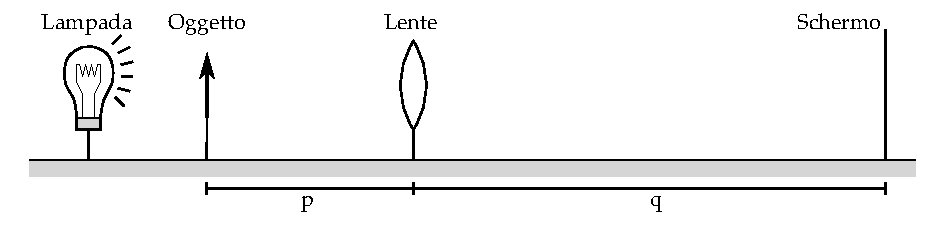
\includegraphics[width=16cm]{drawing.pdf}
    \caption{Schema dell'apparato sperimentale usato per la misura del fuoco della lente convergente.}
    \label{fig:conv}
\end{figure}

\subsection{Fuoco della lente convergente}

Per non appesantire la lettura, nel seguito indicheremo con queste lettere le seguenti quantità (si veda la Figura \ref{fig:conv}):

\begin{equation*}
	p \,=\, \text{distanza tra il centro della lente e la posizione dell'oggetto}
\end{equation*}
\begin{equation*}
	q \,=\, \text{distanza tra il centro della lente e la posizione dell'immagine}
\end{equation*}
\begin{equation*}
	f \,=\, \text{fuoco della lente analizzata}
\end{equation*}
\begin{equation*}
	h \ped{imm} \,=\, \text{altezza dell'immagine sullo schermo}
\end{equation*}
\begin{equation}
	\text{Legge dei punti coniugati:} \qquad \frac{1}{f} \,=\, \frac{1}{p} + \frac{1}{q}
	\label{eq:coniugati}
\end{equation}
\begin{equation}
	\text{Legge del costruttore di lenti:} \qquad \frac{1}{f} \,=\, (n-1)\left(\frac{1}{R\ped{1}}-\frac{1}{R\ped{2}}\right)
	\label{eq:costruttore}
\end{equation}


Come primo obbiettivo ci siamo posti di calcolare il fuoco della lente convergente e l'ingrandimento della lente per diversi valori di $p$ e $q$. Per ottenere questo riultato abbiamo misurato per dodici valori di $p$ al variare di $q$. Questo è stato fatto tenendo ferma la sorgente luminosa, incrementando di volta in volta la distanza tra la lente e la sorgente luminosa e mettendo a fuoco l'immagine sullo schermo. Si è poi misurata la distanza lente-schermo $q$, la distanza oggetto-lente $p$ e la dimensione $h\ped{imm}$ dell'immagine. Le misure di distanza sono state eseguite con il metro a nastro prestando attenzione a minimizzare l'inclinazione del metro rispetto all'asse ottico. Inoltre la lettura è stata eseguita nel centro della lente. Le misure di dimensione dell'immagine sono invece state eseguite con il calibro ventesimale.

Ovviamente, la distanza oggetto-lente è stata mantenuta maggiore della distanza focale ($p > f$). In caso contrario si avrebbe infatti un immagine virtuale e sarebbe impossibile mettere a fuoco l'immagine sullo schermo.

E' importante sottolineare che nel caso in cui l'immagine si è formata ad una grande distanza dalla lente, riuscire a metterla a fuoco non è stato semplice a causa dell'effetto di profondità di campo. Abbiamo deciso quindi di prendere due misure di $q$, $q_1$ e $q_2$, secondo la seguente procedura. Quando l'immagine era circa a fuoco, abbiamo mosso lo schermo in avanti e in dietro in modo da avere l'immagine leggermente fuori fuoco in entrambe le direzione; abbiamo quindi annotato le due distanze. Siccome è facile vedere quando un oggetto è appena fuori fuoco, facendo la media di questi due valori si ottiene un valore di $q$ più preciso rispetto alla misura diretta.

Una volta ottenuti i valori  di $p$ e $q$, abbiamo calcolato per ognuno il relativo valore di $f$ utilizzando la formula \ref{eq:coniugati} (legge dei punti coniugati). Infine è stata calcolata la media aritmetica dei valori, con la quale abbiamo ottenuto il seguente valore della focale:

\begin{equation}
    f \ped{conv} \,=\, 24 \pm 1 \; \si{\centi\metre}
\end{equation}

Inoltre vogliamo ricavare il valore della magnificazione per ogni coppia $p$ e $q$. Ricordiamo che la magnificazione è il rapporto tra le dimensioni dell'immagine ottenuta ($h \ped{imm}$) rispetto alle dimensioni reali dell'oggetto ($h$). La dimensione dell'oggetto era $h = \SI{9}{\milli\metre}$.

\begin{equation}
	m_{1} \,=\, \frac{h \ped{imm}}{h}
\end{equation}

Infine per avere una verifica della correttezza dei dati registrati, possiamo mettere a confronto il valore della magnificazione trovato empiricamente con quello che si può ricavare dalla seguente relazione:

\begin{equation}
	m_{2} \,=\, \frac{q}{p}
\end{equation}

[Tabella $m_1$, $m_2$, p, q, $h_{imm}$ e incertezze. Forse f?]
% in realtà non so se vuole tutti sti dati, però secondo me è meglio metterceli, perché
% in una relazione scientifica si mettono sempre tutti io dati per permettere agli altri di controllare eventuali
% errori. Comunque almeno m_1 e m_2... FRAPA X BUZZ

Come si può osservare dai dati in tabella i due valori della magnificazione ricavati con entrambi i procedimenti risultano compatibili entro i propri errori. 
% X BUZZ: metti a posto anche il commento qui quando hai fatto la tabella.

\subsection{Aberrazione cromatica relativa alla lente convergente}

Ogni lente è soggetta a un difetto, detto aberrazione cromatica, dovuto al fatto che l'indice di rifrazione del vetro della lente varia al variare della lunghezza d'onda della luce incidente.
Per valutare e osservare il fenomeno dell'aberrazione cromatica, abbiamo calcolato, sempre utilizzando la relazione (\ref{eq:coniugati}), il fuoco della lente convergente usando luce monocromatica rossa e blu. Per ottenere luce monocromatica non abbiamo fatto altro che porre un filtro colorato di fronte alla sorgente luminosa. I valori $p$ e $q$ sono stati presi seguendo lo stesso procedimento adottato per la lente convergente, salvo il fatto che è stato preso solo un valore dei due parametri invece che 12.

Rosso e blu sono stati scelti per massimizzare la differenza tra i fuochi e facilitare le misure; essi si trovano infatti agli estremi opposti dell'intervallo di lunghezze d'onda della luce visibile e quindi i fuochi sono il più distante possibile tra di loro. Inoltre abbiamo mantenuto $p \simeq q$ per facilitare la misura. Infatti se $p$ è piccolo e $q$ grande (come implica la legge dei punti coniugati \ref{eq:coniugati}) la misura è difficile a causa dell'effetto di profondità di campo, metre per $q$ piccoli la distanza tra i fuochi è molto piccola.

Un piccolo accorgimento che è stato preso nell'eseguire questa misura è stato quello di scegliere una distanza $p$ che fosse simile alla distanza $q$.
I risultati da noi ottenuti sono riportati nella tabella sottostante:

[TABELLA!!!]

Come si può notare dai dati in tabella i valori per il fuoco della lente convergente sono differerenti a seconda della lunghezza d'onda (colore) dei raggi luminosi incidenti su quest'ultima. 

\subsection{Aberrazione sferica relativa alla lente convergente}

Per descrivere questo fenomeno diamo un'idea di quello che si intende con:
\begin{itemize}
	\item{Fascio di luce cenrale: è l'insieme dei raggi luminosi che investono la lente convergente nel suo centro;}
	\item{Fascio di luce divergente: e l'insieme dei raggi luminosi che incidono sulla periferia della lente ovvero sulla sezione circolare, più distante dal centro, di quest'ultima;}
\end{itemize}
Adottato lo stesso accorgimento del punto precedente e fissata la distanza $p$ abbiamo esaminato il valore di $q$ selezionando solo il fascio di luce centrale. Questo è stato possibile perchè abbiamo posto sula lente un diaframma che ne oscurava tutta la superficie a parte la sezione centrale. Quindi si poteva supporre che i raggi incidenti formassero un angolo di $\frac{\pi}{2}$ con la superficie.
Successivamente per troare il valore di $q$ relativo al fascio di luce divergente abbiamo posto sulla lente un diaframma, ma con una fenditura circolare distante dal centro, in modo che i raggi incidenti sulla superficie non siano perpendicolari.
Quindi grazie ai valori di $q$ possiamo ora ricavare i valori della focale nei due casi. I isultati sono riportati nela tabella sottostante:

[TABELLA!!!]

Come si può notare per il facio di luce divergente il valore della focale della lene risulta essere minore rispetto al valore ottenuto per i raggi centrali. Questo succede proprio perchè nel secondo caso per i raggi luminosi non era più valida l'approssimazione di raggi parassiali.


\begin{figure}[b!]
	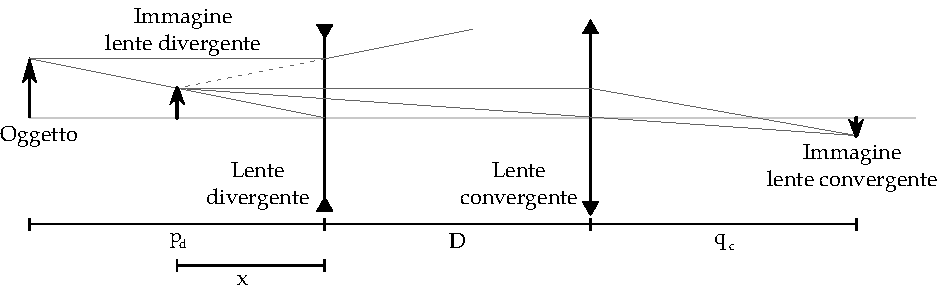
\includegraphics[width=16cm]{drawing2.pdf}
\end{figure}

\subsection{Fuoco della lente divergente}

Dal momento che per una lente divergente l'immagine che si ottiene è un immagine virtuale e non reale, ovvero l'immagine non si forma per intersezione dei raggi reali, ma per il loro prolungamento. Quindi risulterebbe impossibile misurare dirttamente il valre di $q$ usando solamente la lente divergente.
A tal fine abbiamo assemblato un sistema di lenti illustrato nella figura sottostante.

[STESSA FIGURA PRECEDENTE CON AGGIUNTA LA LENTE DIVERGENTE TRA LA SORENTE E LA LENTE DIVERGENTE]

Quindi indicando con:
\begin{itemize}
	\item{$p\ped{d}\,\,$ la distanza tra la sorgente luminosa e il centro della lente divergente;}
	\item{$D\,\,$ la distanza tra le due lenti;}
	\item{$q\ped{c}\,\,$ òa distanza tra il centro della lente convergente e l'immagine;}
	\item{$x\,\,$ la distnza incognita tra il centro della lente divergente e l'immagine data da questa;}
\end{itemize}
Il sistema ideato funziona nel seguente modo: la lente divergente produce un'mmagine virtuale tra la sorgente e se stessa. Qusta immagine diventa quindi il nuovo oggetto per la lente convergente che produce un immagine sullo schermo che noi possiamo vedere. Quindi potendo misurare tutti i parametri sopraelencati ad eccezzione di $x$ e $f\ped{d}$ (focale lente divergente) e conoscendo $f\ped{c}$ (focale lente convergente) risolvendo questo semplice sistema:

%\begin{equation}
%	\frac{1}{f\ped{d}} \,=\, \frac{1}{p\ped{d}} + \frac{1}{x}
%	\frac{1}{f\ped{c}} \,=\, \frac{1}{(D + x)} + \frac{1}{q\ped{c}}
%\end{equation}
\begin{equation}
 \left\{
  \begin{aligned}
    \frac{1}{f\ped{d}} & \,=\, \frac{1}{p\ped{d}} + \frac{1}{x}\\
    \frac{1}{f\ped{c}} & \,=\, \frac{1}{(D + x)} + \frac{1}{q\ped{c}}
  \end{aligned}
\right.
\end{equation}
%
possiamo ottenere i valori di $x$ e $f\ped{d}$. Inoltre per ottenere un valore più accurato di $f\ped{d}$ abbiamo tenuta ferma la distanza $p\ped{d}$ e abbiamo variato la distanza $D$ e quindi anche $q\ped{c}$, per tre volte. Quindi per ognuna tripletta abbiamo sfruttato la relazione (\ref{coniugati}) e abbiamo ottenuto tre valori di $f\ped{d}$. Facendone pertanto la media otterremo un valore più accurato di $f\ped{d}$
Quindi abbiamo ottenuto che:

\begin{equation}
	x \,=\, XXX \qquad \text{e} \qquad f\ped{d} \,=\, XXX
\end{equation}

Infine anche per questa lente abbiamo calcolato il valore della magnificazione. Quindi con i valori di $p\ped{d}$ e di $x$ sfruttando la relazione:
\begin{equation}
	|m| \,=\, \frac{x}{p\ped{d}} \,=\,
\end{equation}
dove $x$ non è altro che il valore di $q\ped{d}$
%Ovvero conoscendo il valore di $m$ per la lente convergente abbiamo sfruttato la relazione:
%\begin{equation}
%	m \'=\' \frac{h\ped{imm}}{h\ped{ogg}} 
%\end{equation}
%e quindi abbiamo ricavato il valore dell'altezza dell'oggetto per la ente converegente, che però risulta essere nient'altro che l'altezza dell'immagine della lente divergente. Pertanto per ricavare la magnificazione di quest'ultima abbiamo applicato nuovamente la relazione:
%\begin{equation}
%	m \'=\' \frac{h\ped{ogg}}{h} 
%\end{equation}
%e abbiamo ottenuto che $m \'=\' XXX$ 

\subsection{indice di rifrazione della lente convergente}

Per ricavare il valore dell'indice di rifrazione della lente convergente ($n$) non dobbiamo fare altro che sfruttare la relazione (\ref{costruttore}). A tal fine abbiamo usato il calibro per misurare i diametro della lente, il suo spessore al centro e quello al bordo. Tutti questi dati sono necessari in quanto nella legge sopracitata sono necessari i valori di $R\ped{1}$ e $R\ped{2}$ che nel nostro caso hanno valore uguale. $R\ped{1}$ e $R\ped{2}$ non sono altro che le distanze tra il centro della lente e la superficie della stessa. Quindi il problema di ricavare $R\ped{1}$ e $R\ped{2}$ si riduce ad un semplice problema di gometria elementare.
Il valore ottenuto di $R$ e: $R \,=\, XXX$.
Quindi per concludere il vaore dell'indice di rifrazione ($n$) della lente convergente risulta essere:

\begin{equation}
	n \,=\, XXX
\end{equation}







